\documentclass[12pt,a4paper,openany]{report}
%%%% JNLP 
\usepackage{lmodern}
\usepackage{xcolor}
\usepackage[utf8]{inputenc}
\usepackage[T1]{fontenc}
\usepackage[francais]{babel}
\usepackage[top=1.7cm, bottom=1.7cm, left=1.5cm, right=1.5cm]{geometry}
\usepackage{pdfpages}
\usepackage{listingsutf8} \usepackage{fancyhdr}
\usepackage{multido}
\usepackage{multicol}
\usepackage{amssymb}
\usepackage{tikz}
\usepackage{ifthen}
\usepackage{makeidx}
\usepackage{float}
\usepackage[urlbordercolor={1 1 1}, linkbordercolor={1 1 1}, urlcolor=blue]{hyperref}

\newcommand{\headGauche}{}
\newcommand{\headCentre}{}
\newcommand{\headDroite}{}
%\newCommand{\footGauche}{} Université paul sabatier Toulouse III
\newcommand{\footCentre}{}
%\newCommand{\footDroite}{} Numéro de page
\newcommand{\premierDestinataire}{Monsieur Max Chevalier}
\newcommand{\rolePremierDestinataire}{Resonsable projet}

\newcommand{\secondDestinaire}{Madame Caroline Kross}
\newcommand{\roleSecondDestinaire}{Tutrice}

\newcommand{\troisiemeDestinaire}{Monsieur Thierry Millan}
\newcommand{\roleTroisiemeDestinaire}{Client}

\newcommand{\quatriemeDestinaire}{}
\newcommand{\roleQuatriemeDestinaire}{}

\newcommand{\cinquiemeDestinaire}{}
\newcommand{\roleCinquiereDestinaire}{}
\newcommand{\titreDocument}{Les plans et les cahiers de tests}


\date{\today}

\chead{\headCentre}
\rhead{\headDroite}
\lhead{\headGauche}
\makeindex
\lfoot{Université Paul Sabatier Toulouse III}
\rfoot{--~\thepage~--}
\cfoot{\footCentre}
\makeglossary
\makeatletter
\def\clap#1{\hbox to 0pt{\hss #1\hss}}%
\def\ligne#1{%
\hbox to \hsize{%
\vbox{\centering #1}}}%
\def\haut#1#2#3{%
\hbox to \hsize{%
\rlap{\vtop{\raggedright #1}}%
\hss
\clap{\vtop{\centering #2}}%
\hss
\llap{\vtop{\raggedleft #3}}}}%
\def\bas#1#2#3{%
\hbox to \hsize{%
\rlap{\vbox{\raggedright #1}}%
\hss \clap{\vbox{\centering #2}}%
\hss
\llap{\vbox{\raggedleft #3}}}}%
\def\maketitle{%
\thispagestyle{empty}\vbox to \vsize{%
\haut{}{\@blurb}{}
\begin{flushleft}
	\vspace{1cm}
	Antoine de \bsc{Roquemaurel}\\ 
	Mathieu \bsc{Soum}\\
	Geoffroy \bsc{Subias}\\
	Marie-Ly \bsc{Tang}\\
	\textit{Groupe B}\\
\end{flushleft}
\begin{flushright}
	\vspace{-3cm}
	\ifthenelse{\equal{\premierDestinataire}{}}{
	}
	{
		Pour \premierDestinataire(\rolePremierDestinataire)\\
	}
	\ifthenelse{\equal{\secondDestinaire}{}}{
	}
	{
		Pour \secondDestinaire(\roleSecondDestinaire)\\
	}
	\ifthenelse{\equal{\troisiemeDestinaire}{}}{
	}
	{
		Pour \troisiemeDestinaire(\roleTroisiemeDestinaire)\\
	}
	\ifthenelse{\equal{\quatriemeDestinaire}{}}{
	}
	{
		Pour \quatriemeDestinaire(\roleQuatriemeDestinaire)\\
	}
	\ifthenelse{\equal{\cinquiemeDestinaire}{}}{
	}
	{
		Pour \cinquiemeDestinaire(\roleCinquiereDestinaire)\\
	}
\end{flushright}
\vfill
\vspace{1cm}
\begin{flushleft}
\usefont{OT1}{ptm}{m}{n}
\huge \@title
\end{flushleft}
\par
\hrule height 4pt
\par
\begin{flushright}
\usefont{OT1}{phv}{m}{n}
\Large \@author
\par
\end{flushright}
\vspace{1cm}
\vfill
\vfill
\bas{}{\@location, le \@date}{}
}%
\cleardoublepage
}
\def\date#1{\def\@date{#1}}
\def\author#1{\def\@author{#1}}
\def\title#1{\def\@title{#1}}
\def\location#1{\def\@location{#1}}
\def\blurb#1{\def\@blurb{#1}}
\date{\today}
\author{}
\title{}
\location{Amiens}\blurb{}
\makeatother
\title{\titreDocument}
\author{Bibliothèque d'objets graphiques UML}

\location{Toulouse}
\blurb{%
Université Paul Sabatier -- Toulouse III\\
IUT A - Toulouse Rangueil\\
\textbf{Projet tuteuré}\\[1em]
}%



\pagestyle{fancy}

\definecolor{gris1}{gray}{0.40}
\definecolor{gris2}{gray}{0.55}
\definecolor{gris3}{gray}{0.65}
\definecolor{gris4}{gray}{0.50}
\definecolor{vert}{rgb}{0,0.4,0}
\definecolor{bleu1}{rgb}{0,0,0.8}
\definecolor{bleu2}{rgb}{0,0.2,0.6}
\definecolor{bleu3}{rgb}{0,0.2,0.2}


\lstdefinelanguage{algo}{%
   morekeywords={%
    %%% couleur 1
		importer, programme, glossaire, fonction, procedure, constante, type, 
	%%% IMPORT & Co.
		si, sinon, alors, fin, tantque, debut, faire, lorsque, fin lorsque, 
		declenche, declencher, enregistrement, tableau, retourne, retourner, =, 
		/=, <, >, traite,exception, 
	%%% types 
		Entier, Reel, Booleen, Caractere, Réél, Booléen, Caractère,
	%%% types 
		entree, maj, sortie,entrée,
	%%% types 
		et, ou, non,
	},
  sensitive=true,
  morecomment=[l]{--},
  morestring=[b]',
}

\lstset{language=algo,
    %%% BOUCLE, TEST & Co.
      emph={importer, programme, glossaire, fonction, procedure, constante, type},
      emphstyle=\color{bleu2},
    %%% IMPORT & Co.  
	emph={[2]
		si, sinon, alors, fin , tantque, debut, faire, lorsque, fin lorsque, 
		declencher, retourner, et, ou, non,enregistrement, retourner, retourne, 
		tableau, /=, <, =, >, traite,exception
	},
      emphstyle=[2]\color{bleu1},
    %%% FONCTIONS NUMERIQUES
      emph={[3]Entier, Reel, Booleen, Caractere, Booléen, Réél, Caractère},
      emphstyle=[3]\color{gris1},
    %%% FONCTIONS NUMERIQUES
      emph={[4]entree, maj, sortie, entrée},	
      emphstyle=[4]\color{gris1},
}
\lstdefinelanguage{wl}{%
   morekeywords={%
    %%% couleur 1
		importer, programme, glossaire, fonction, procedure, constante, type, 
	%%% IMPORT & Co.
		si, sinon, alors, fin, TANTQUE, tantque, FIN, PROCEDURE, debut, faire, lorsque, 
		fin lorsque, declenche, declencher, enregistrement, tableau, retourne, retourner, =, 
		/=, <, >, traite,exception, 
	%%% types 
		Entier, Reel, Booleen, Caractere, Réél, Booléen, Caractère,
	%%% types 
		entree, maj, sortie,entrée,
	%%% types 
		et, ou, non,
	},
  sensitive=true,
  morecomment=[l]{//},
  morestring=[b]',
}

\lstset{language=wl,
    %%% BOUCLE, TEST & Co.
      emph={importer, programme, glossaire, fonction, procedure, constante, type},
      emphstyle=\color{bleu2},
    %%% IMPORT & Co.  
	emph={[2]
		si, sinon, alors, fin , tantque, debut, faire, lorsque, fin lorsque, 
		declencher, retourner, et, ou, non,enregistrement, retourner, retourne, 
		tableau, /=, <, =, >, traite,exception
	},
      emphstyle=[2]\color{bleu1},
    %%% FONCTIONS NUMERIQUES
      emph={[3]Entier, Reel, Booleen, Caractere, Booléen, Réél, Caractère},
      emphstyle=[3]\color{gris1},
    %%% FONCTIONS NUMERIQUES
      emph={[4]entree, maj, sortie, entrée},	
      emphstyle=[4]\color{gris1},
}
\lstdefinelanguage{css}{%
   morekeywords={%
    %%% couleur 1
		background, image, repeat, position, index, color, border, font, 
		size, url, family, style, variant, weight, letter, spacing, line, 
		height, text, decoration, align, indent, transform, shadow, 
		background, image, repeat, position, index, color, border, font, 
		size, url, family, style, variant, weight, letter, spacing, line, 
		height, text, decoration, align, indent, transform, shadow, 
		vertical, align, white, space, word, spacing,attachment, width, 
		max, min, margin, padding, clip, direction, display, overflow,
		visibility, clear, float, top, right, bottom, left, list, type, 
		collapse, side, empty, cells, table, layout, cursor, marks, page, break,
		before, after, inside, orphans, windows, azimuth, after, before, cue, 
		elevation, pause, play, during, pitch, range, richness, spek, header, 
		numeral, punctuation, rate, stress, voice, volume,
	%%% types 
		left, right, bottom, top, none, center, solid, black, blue, red, green,
	},
  sensitive=true,
  sensitive=true,
  morecomment=[s]{/*}{*/},
  morestring=[b]',
}
\lstset{language=css,
    %%% BOUCLE, TEST & Co.
      emph={
		background, image, repeat, position, index, color, border, font, 
		size, url, family, style, variant, weight, letter, spacing, line, 
		height, text, decoration, align, indent, transform, shadow, 
		background, image, repeat, position, index, color, border, font, 
		size, url, family, style, variant, weight, letter, spacing, line, 
		height, text, decoration, align, indent, transform, shadow, 
		vertical, align, white, space, word, spacing,attachment, width, 
		max, min, margin, padding, clip, direction, display, overflow,
		visibility, clear, float, top, right, bottom, left, list, type, 
		collapse, side, empty, cells, table, layout, cursor, marks, page, break,
		before, after, inside, orphans, windows, azimuth, after, before, cue, 
		elevation, pause, play, during, pitch, range, richness, spek, header, 
		numeral, punctuation, rate, stress, voice, volume,
	  },
      emphstyle=\color{bleu2},
    %%% FONCTIONS NUMERIQUES
      emph={[3]
		left, right, bottom, top,none, solid, black, blue, green,
		  },
      emphstyle=[3]\color{bleu3},
    %%% FONCTIONS NUMERIQUES
}
\lstdefinelanguage{SQL}{%
   morekeywords={%
    %%% couleur 1
	INSERT, if, end, begin,UPDATE, DELETE, SET, WHERE, 
	CREATE, OR, REPLACE, AND, FROM, SELECT, VIEW, TRIGGER, AS, GROUP,
	BY, ORDER, after, for, each, then, else, of, on
	},
  sensitive=true,
  morecomment=[l]{--},
  morestring=[b]',
}

\lstset{language=SQL,
    %%% BOUCLE, TEST & Co.
      emph={INSERT, UPDATE, DELETE, WHERE, SET, GROUP, BY, ORDER},
      emphstyle=\color{bleu2},
    %%% IMPORT & Co.  
	emph={[2]
		if, end, begin, then, for, each, else, after, of, on
	},
      emphstyle=[2]\color{bleu1},
    %%% FONCTIONS NUMERIQUES
      emph={[3]Entier, Reel, Booleen, Caractere, Booléen, Réél, Caractère},
      emphstyle=[3]\color{gris1},
    %%% FONCTIONS NUMERIQUES
      emph={[4]entree, maj, sortie, entrée},	
      emphstyle=[4]\color{gris1},
}
\lstset{ % general style for listings 
   numbers=left 
   , literate={é}{{\'e}}1 {è}{{\`e}}1 {à}{{\`a}}1 {ê}{{\^e}}1 {É}{{\'E}}1 {ô}{{\^o}}1 {€}{{\euro}}1{°}{{$^{\circ}$}}1 {ç}{ {c}}1 {î}{{\^i}}1
	, extendedchars=\true
   , tabsize=2 
   , frame=single 
   , breaklines=true 
   , basicstyle=\ttfamily 
   , numberstyle=\tiny\ttfamily 
   , framexleftmargin=0mm 
   , xleftmargin=0mm 
   , captionpos=b 
	, keywordstyle=\color{bleu2}
	, commentstyle=\color{vert}
	, showstringspaces=false
	, extendedchars=true
	, mathescape=true
} 

\addto\captionsfrench{%
	\renewcommand{\listfigurename}{Liste des figures}%
}
\begin{document}
	\maketitle
	\newpage
	\setcounter{tocdepth}{3}
	\setcounter{secnumdepth}{3}
	\chapter*{Avant-propos}
\nouveauChapitre
\addcontentsline{toc}{chapter}{Avant-propos}
\section*{Présentation du projet}
\addcontentsline{toc}{section}{Présentation du projet}
	LibUML est une 
	\glo{bibliothèque}{Bibliothèque}{Composant programmé dans un langage donné fournissant des méthodes permettant d'effectuer des tâches voulut} 
	d'objets graphiques représentant les différents éléments de modélisation de la norme 
	\glo{UML}{UML}{(Unified Modeling Language) Langage de modélisation graphique à base de pictogramme.  Il est apparu dans le monde du génie logiciel dans le cadre de la conception orientée objet. Ce langage est composé de différents diagrammes, allant du développement à la simple analyse des besoins.} 
	2\footnote{Unified Modelling Language}.
	Celle-ci à été développé dans le cadre des projets tuteurés à l'IUT\footnote{Institut Universitaire de Technologies} 'A' de Toulouse. 
	Nous l'avons développée en \glo{Java}{Java}{Langage de programmation orienté objet moderne, il compile le programme pour ensuite l'exécuter sur une machine Java, ainsi le programme une fois compilé peut être exécuté sur différentes plateformes (Windows, Linux, Mac OS X, \ldots).} 
	et conçut comme une bibliothèque pouvant être utilisée dans des programmes Java comme composant. 
	Vous pouvez vous en servir pour développer un outil complet de modélisation UML par exemple.
	\paragraph{}	
	Cette bibliothèque permet de faire différentes choses dans le cadre de la conception UML, une fois la
	que vous aurez compris le fonctionnement de libUML vous pourrez:
	\begin{itemize}
		\item Créer des éléments de modélisation 
			\begin{itemize}
				\item Acteur actif ou passif
				\item Traitement
				\item Cas d'utilisation
				\item Classe
			\end{itemize}
		\item Relier ses composants via différents types de flèches
			\begin{itemize}
				\item Agrégation
				\item Composition
				\item Association binavigable ou mononavigable
				\item Messages synchrones ou asynchrones
				\item Généralisation
			\end{itemize}
		\item Supprimer des éléments et flèches
		\item Modifier le contenu des éléments et flèches
		\item Redimensionner les éléments de modélisation
	\end{itemize}
	\paragraph{}
Ce document à pour but de vous présenter le fonctionnement de la bibliothèque UML et de son démonstrateur. 

\section*{Présentation du groupe}
\addcontentsline{toc}{section}{Présentation du groupe}
	Notre groupe projet est composé de quatre étudiants de deuxième année de DUT Informatique à l'IUT 'A' de Toulouse, voici la composition de l'équipe: 
	\begin{itemize}
		\item Antoine de \bsc{Roquemaurel} 
		\item Mathieu \bsc{Soum} 
		\item Geoffroy \bsc{Subias}
		\item Marie-Ly \bsc{Tang} 
	\end{itemize}
	\section*{Téléchargements}
\addcontentsline{toc}{section}{Téléchargements}
	Nous vous avons envoyé deux archives zip par email, une contenant le projet Netbeans de la bibliothèque et du démonstrateur et une contenant la bibliothèque.
	\subsubsection*{Bibliothèque et démonstrateur}
	La première archive est donc un projet netbeans, cette archive contient notre bibliothèque et ses tests associés, le démonstrauteur mais
	également la bibliothèque \texttt{JGraphx} qui est indispensable au bon fonctionnement de notre bibliothèque. Nous ne garantissons le bon fonctionnement 
	de la bibliothèque qu'avec la version de \texttt{JGraphx} 1.8, celle-ci n'ayant pas été testé avec des versions différentes.

	Le projet netbeans de notre bibliothèque est également disponible en ligne, si vous souhaitez la télécharger de nouveau, elle est donc disponible à l'adresse suivante: \\
	$\rhd$ \url{http://telechargements.joohoo.fr/libUML/libUML-netbeans.zip}\\
	$\rhd$ \url{http://telechargements.joohoo.fr/libUML/JGraphX-1.8.jar}\\
	
	\subsubsection*{Documentation}
	Toute la documentation du projet est sous format \bsc{HTML}\footnote{HyperText Markup Language}, celle-ci ayant été générée grâce à Javadoc.

	Si dans ce manuel nous parlons d'une méthode et que vous n'en comprenez pas l'intéret, vous pouvez aller la chercher dans la documentation, pour chaque classe,
	le fonctionnement global de la classe est expliquée, l'utilité de chaque attribut, de chaque méthode, et ce que vous devez mettre dans les différents paramètres 
	des méthodes.  
	\paragraph{}
	Nous vous avons remis un .zip par email contenant quatre dossiers de documentation:
	\begin{itemize}
		\item La documentation privée de la \textit{bibliothèque} (Toutes les méthodes et tous les attributs)
		\item La documentation publique de la \textit{bibliothèque} (Seuls les méthodes et attributs publiques ou protégées)
		\item La documentation privée du \textit{démonstrateur} (toutes les méthodes du démonstrateur) 
		\item La documentation des \textit{tests unitaires} (Toutes les méthodes de tests)
	\end{itemize}
	\paragraph{}
	Celle ci est également disponible en ligne aux adresses suivantes: \\
	$\rhd$ \url{http://documentation.joohoo.fr/libUML/bibliothequePrivee/index.html}\\
	$\rhd$ \url{http://documentation.joohoo.fr/libUML/bibliothequePublique/index.html}\\
	$\rhd$ \url{http://documentation.joohoo.fr/libUML/demonstrateurPrivee/index.html}\\\label{docDemonstrateur}
	$\rhd$ \url{http://documentation.joohoo.fr/libUML/testsUnitaires/index.html}\\
	\paragraph{}
	Vous pouvez également accéder à la documentation de \texttt{JGraphX}, cela peut vous être utile dans certains cas.\\
	$\rhd$ \url{http://documentation.joohoo.fr/JGraphX/index.html}\\ 


	\newpage
\section*{Fonctionnement du document}
\addcontentsline{toc}{section}{Fonctionnement du document}
Ce document est un document expliquant notre approche pour développer une bibliothèque d'objets graphiques UML.\\

Dans ce dossier, vous pourrez repérer diverses notations, cette partie a pour but de vous expliquer les notations afin
que vous puissiez lire en toute sérénité.
\subsubsection*{Le glossaire}
Un mot dans le glossaire a une police particulière, vous pourrez savoir qu'un mot est dans le glossaire lorsque vous repérerez un mot avec la police suivante: 
\policeGlossaire{leMotDansLeGlossiare}. Si vous voyez cette police, vous pouvez donc vous référez à l'annexe \ref{glossaire} page \pageref{glossaire}.
\subsubsection*{Les noms de méthode, d'attribut ou de classe}
Les mots se référant à un nom présent dans du code ont une police particulière, une police type ``machine à écrire'', si vous voyez la police suivante, c'est que c'est un nom 
de méthode, d'attribut ou de classe: \texttt{uneFonction}.
\subsubsection*{Les noms de paquetage}
Les noms de paquetage utiliseront une police particulière, afin que l'on puisse les différencier d'une classe ou d'une méthode, vous les trouverez 
comme suit : \policePackage{unPaquetage}.
\subsubsection*{Les notes de bas de page}
Nous utilisons régulièrement des notes de bas de pages, pour donner un acronyme, pour expliquer plus en détail une notion, ces notes de bas de pages sont un numéro
en exposant, vous trouverez la note correspondante en bas de la page courante, comme ceci\footnote{Ceci est une note de bas de page}.
\subsubsection*{Les liens hypertextes}
Dans le document, nous pouvons faire référence à un lien d'un site web, tous les liens seront donc symbolisés par une petite puce, et une police particulière comme ceci:\\
	$\rhd$ \url{http://monLien.fr/index.html}\\
	Une liste de tous les liens présents dans le document est accessible en annexe \ref{listeLiens} page \pageref{listeLiens}.


	\tableofcontents
	\newpage
	\chapter{Les plans de tests}
	\section{Les plans de non régression}
	Notre projet est de développé une \glo{bibliothèque}{Bibliothèque}{Un composant indépendant fournissant des méthodes déjà implémentées, facilitant le développement de d'une application plus importante.} \glo{UML}{UML}{(Unified Modeling Language) Langage de modélisation graphique à base de pictogramme. Il est apparu dans le monde du génie logiciel dans le cadre de la conception orientée objet. Ce langage est composé de différents diagrammes, allant du développement à la simple analyse des besoins. } \footnote{Unified Modeling Language}, aucun système n'existant
	au départ, il est donc inutile de faire un test de non régression étant donné que nous ne continuons pas un système, il n'y aura pas 
	de régression.
	\section{Les tests de validation}
	Nous avons développé un \glo{démonstrateur}{Démonstrateur}{Un démonstrateur est un logiciel simple, permettant de montrer les possibilités d'une bibliothèque} qui utilise notre bibliothèque et qui fait office de test de validation. Il nous permet de vérifier que toutes les attentes du client sont respectés. \\
		Avec ce démonstrateur, nous pouvons montrer au client les différentes possibilités de la bibliothèque, ainsi qu'un exemple d'utilisation.

		\subsection{Jeux d'essais}
		\subsubsection{Dessiner un diagramme complet}
		Nous avons effectués plusieurs jeux d'essais, le but est de pouvoir dessiner un pour chacun des types de diagrammes demandés par le client,
		un diagramme utilisant tous les composant de la norme UML 2.0 et respectant cette même norme, ceci pour chacun des diagrammes 
		demandés par notre client. 
		\begin{itemize}
			\item Dessiner un \glo{diagramme de classe}{Diagramme de classe}{Schéma utilisé en génie logiciel pour représenter les classes et les interfaces des systèmes ainsi que les différentes relations entre celles-ci.}.
			\item Dessiner un \glo{diagramme de séquence}{Diagramme de séquence}{ Représentation graphique des interactions entre les acteurs et le système selon un ordre chronologique. Ce diagramme est inclus dans la partie dynamique d'UML.}.
			\item Dessiner un \glo{diagramme de cas d'utilisation}{Diagramme de cas d'utilisation} {Représentation graphique permettant de décrire les intéractions entre les acteurs et le système.}.
		\end{itemize}
	
		\subsubsection{Respecter les contraintes d'ajout d'éléments}
		Pour chacun des diagrammes, les contraintes doivent être respectés, ainsi en fonction du type de diagramme, certains éléments ne doivent pas pouvoir
		être inséré. Voici la liste des éléments autorisés en fonction du type de diagramme.
		\begin{multicols}{2}
		\paragraph{Diagramme de cas d'utilisation}
		\begin{itemize}
			\item Cas d'utilisation
			\item Acteur actif
		\end{itemize}
		\paragraph{Diagramme de classe}
		\begin{itemize}
			\item Classe
			\item Interface
		\end{itemize}
		\paragraph{Diagramme de séquence}
		\begin{itemize}
			\item Traitement
			\item Acteur actif 
			\item Acteur passif
			\item Ligne de vie 
		\end{itemize}
		\end{multicols}

		\subsubsection{Respecter les contraintes de liaisons d'éléments}
		Nous devons également respecter les contraintes de liaison entre les différents éléments. Ainsi voici la liste des liaisons possible.
		\begin{multicols}{2}
		\paragraph{Diagramme de classe}	
		\begin{itemize}
			\item Entre deux classes
				\begin{itemize}
					\item Agrégation
					\item Composition
					\item Association
					\item Spécialisation
				\end{itemize}
			\item Entre une classe et une interface
				\begin{itemize}
					\item Spécialisation
					\item Dépendance fonctionnelle 
						\\ \\
				\end{itemize}
		\end{itemize}
		\paragraph{Diagramme de cas d'utilisation}	
		\begin{itemize}
			\item Entre un acteur un cas d'utilisation
				\begin{itemize}
					\item Association
				\end{itemize}
			\item Entre deux cas d'utilisations
				\begin{itemize}
					\item Dépendance fonctionnelle
				\end{itemize}
		\end{itemize}
		\paragraph{Diagramme de séquence}
		\begin{itemize}
			\item Entre deux traitements
				\begin{itemize}
					\item Dépendance fonctionnelle
					\item Déclenchements
				\end{itemize}
		\end{itemize}
		\end{multicols}
		\subsection{Résultats obtenus}
		Nous vérifierons que les diagrammes sont bien réalisés, qu'il n'y a aucune erreur, et qu'ils correspondent aux besoins du client.\\
		Également, nous vérifierons que nous ne pouvons pas relier ou ajouter des éléments non autorisés par la norme UML 2.0.

	\section{Les tests d'intégration}
		Nous avons développé un démonstrateur qui utilise notre bibliothèque et qui fait office de test d'intégration démontrant que notre système
		est utilisable en tant que composant par un logiciel extérieur. Il nous permet également de montrer au client les possibilités de notre bibliothèque.

		\subsection{Les composants à tester}
			Notre bibliothèque d'objet graphique en tant que composant de notre démonstrateur.

			\subsection{Les jeux d'essais}
			Dessiner un diagramme de classe, un diagramme de séquence ainsi qu'un diagramme de cas d'utilisation chacun utilisant tous les objets graphiques 
			possibles. \\
			Une fois ces diagrammes dessinés, nous testerons la suppression\footnote{La suppression d'un élément devant supprimer les liens de l'élément supprimé},
			l'ajout de méthodes et d'attributs dans une classe, ainsi que la modification de données.

			\subsection{Les résultats attendus}
			Représentation graphique des différents diagrammes respectant les normes UML 2.0 avec possibilité d'ajout ou de suppression de données.
			\newpage
	\section{Les tests unitaires}
	Les tests unitaires servent à tester chacune des méthodes de notre bibliothèque.\\
	Nous avons utiliser \glo{JUnit}{JUnit}{Bibliothèque permettant de créer des tests unitaires simplement} pour tester toutes les méthodes de notre bibliothèque. Les tests sont validés si 
	la bibliothèque \texttt{JUnit} nous indique que tous les tests passent et ne posent pas de problème.
	La description des tests unitaires est disponible sous format Javadoc à l'annexe \ref{junitdoc} page \pageref{junitdoc}.
	Elle est également disponible sous format HTML à l'adresse suivante: \\
	$\rhd$ \url{http://documentation.joohoo.fr/libUML/junitTests/index.html}\\
		
	\section{Le test de charges}
		\subsection{Le jeux d'essai}
		Le test de charge permet de savoir si la création d'un grand nombre d'élément graphique ne posera pas de problème. 
		Ainsi, nous allons créer les éléments suivants dans un diagramme sans contraintes.
		\begin{itemize}
			\item 20 Classes
			\item 20 Cas d'utilisation
			\item 20 Traitements
			\item 20 Acteurs actifs
			\item 20 Acteurs passifs
			\item 20 interface 
			\item 60 liens
		\end{itemize}
		Une fois ces éléments suivants créer, nous supprimerons 40 éléments, qui devront supprimer les liens reliés aux éléments.
		\subsection{Les résultats attendus}
		Aucune exception, les éléments ont été bien créer et certains éléments ont été supprimés avec les liens.
	\chapter{Les cahiers de tests}	
	\section{Création du démonstrateur}
	Pour les tests de validation, nous avons donc créer un démonstrateur, ce démonstrateur à évolué tout au long du développement de la bibliothèque UML, 
	lorsque nous rajoutions des éléments dans la bibliothèque, nous modifions le démonstrateur pour pouvoir les intégrer.
		\begin{figure}[H]
			\centering
			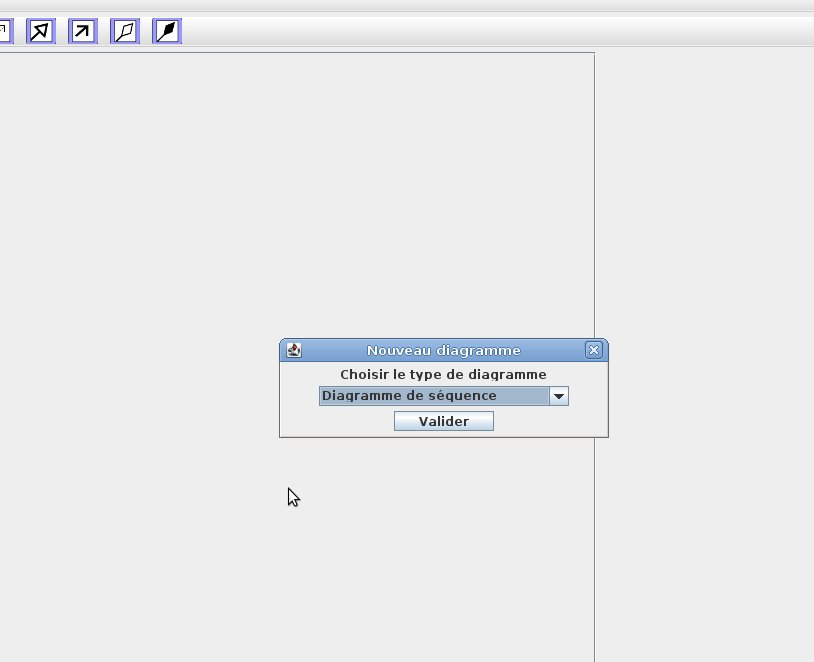
\includegraphics[width=18cm]{choixDiagramme.jpg}
			\caption{Ouverture du démonstrateur (Choix du type de diagramme)}
		\end{figure}
	\newpage
	\section{Les tests de validation}
		\subsection{Dessiner un diagramme de cas d'utilisation}
		\begin{figure}[H]
			\centering
			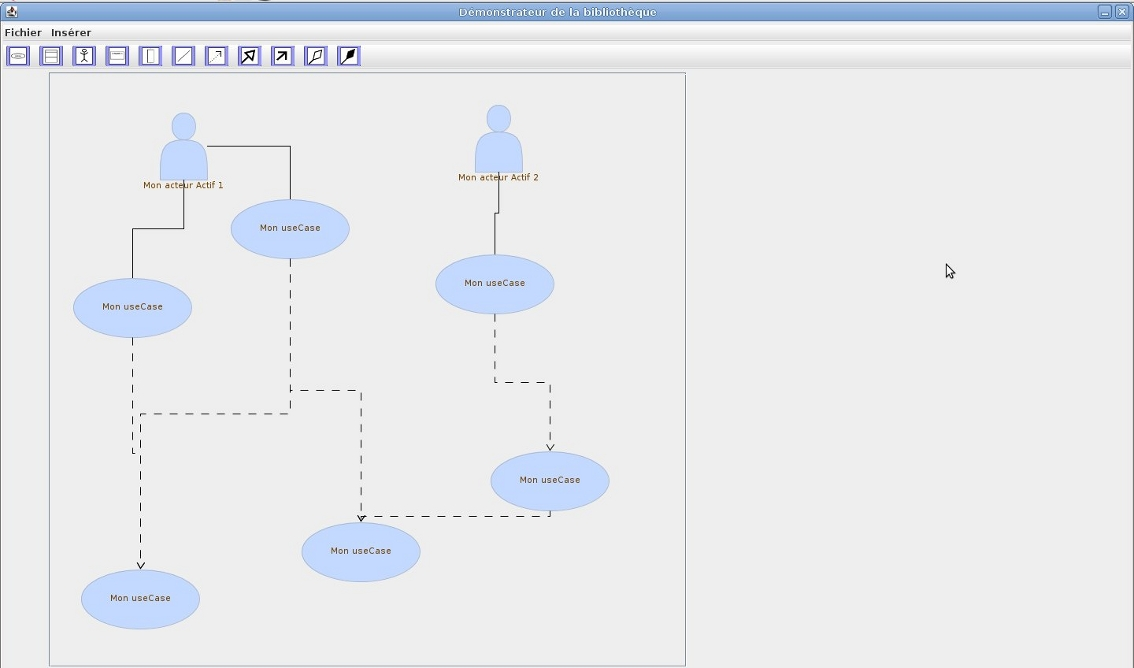
\includegraphics[width=16cm]{validation3.jpg}
			\caption{Création d'un diagramme de cas d'utilisation simple}
			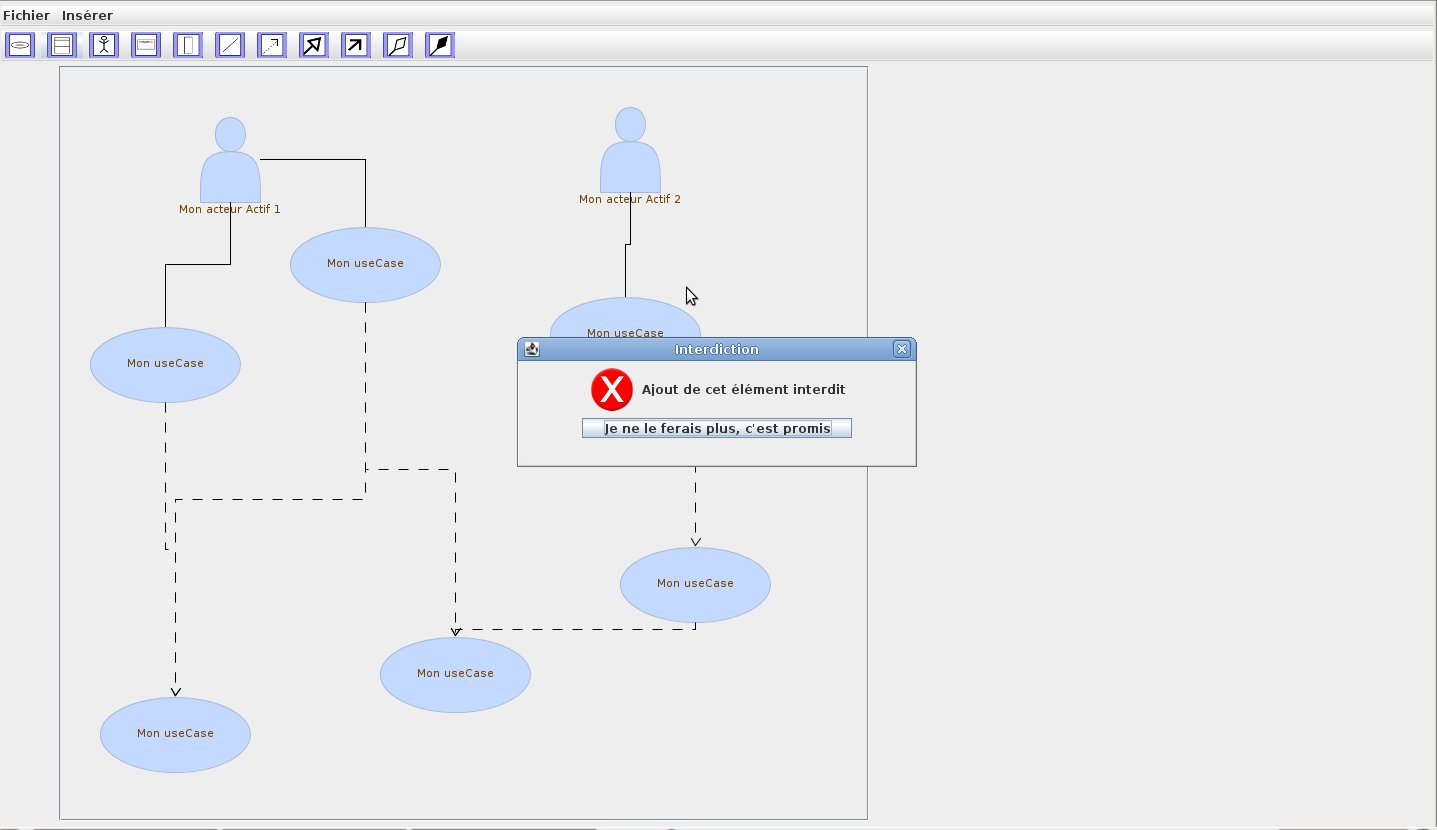
\includegraphics[width=16cm]{validation4.jpg}
			\caption{Validation de l'interdiction d'ajouter des éléments non autorisés}
		\end{figure}
		\subsection{Dessiner un diagramme de classe}
		\begin{figure}[H]
			\centering
			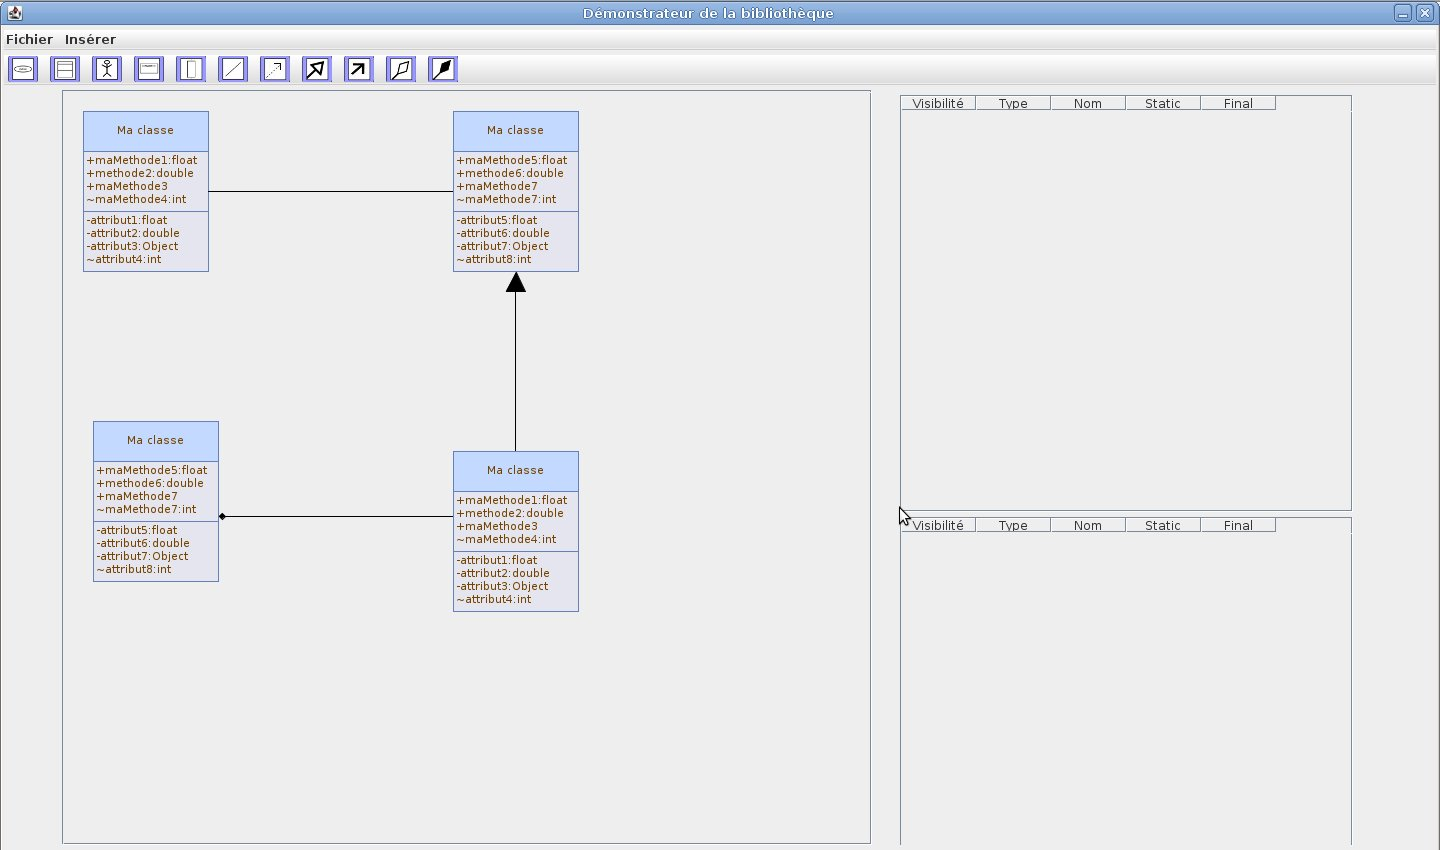
\includegraphics[width=18cm]{validation1.jpg}
			\caption{Création d'un diagramme de classe simple}
			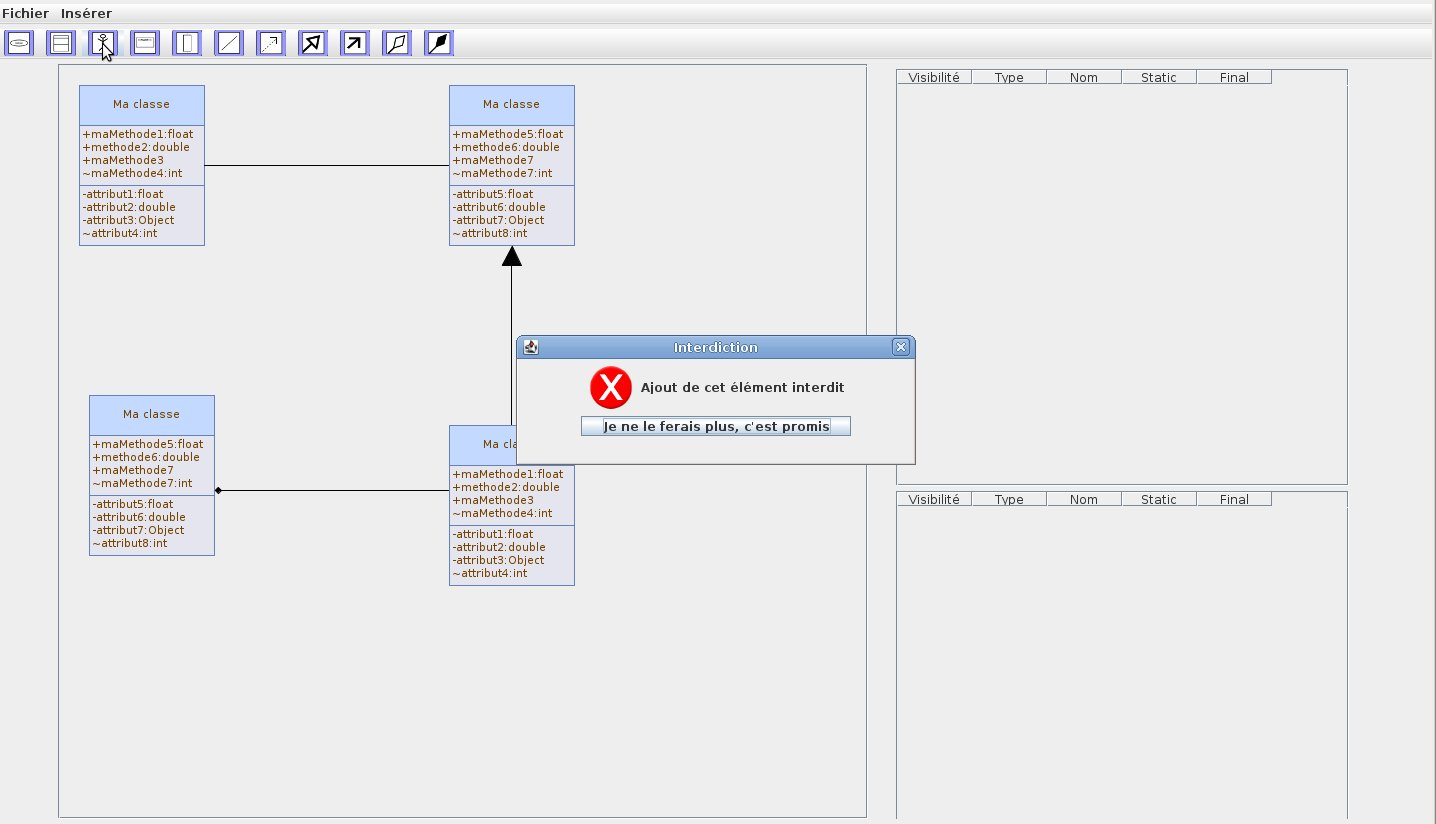
\includegraphics[width=18cm]{validation2.jpg}
			\caption{Validation de l'interdiction d'ajouter des éléments non autorisés}
		\end{figure}
		\subsection{Dessiner un diagramme de séquence}
		\begin{figure}[H]
			\centering
			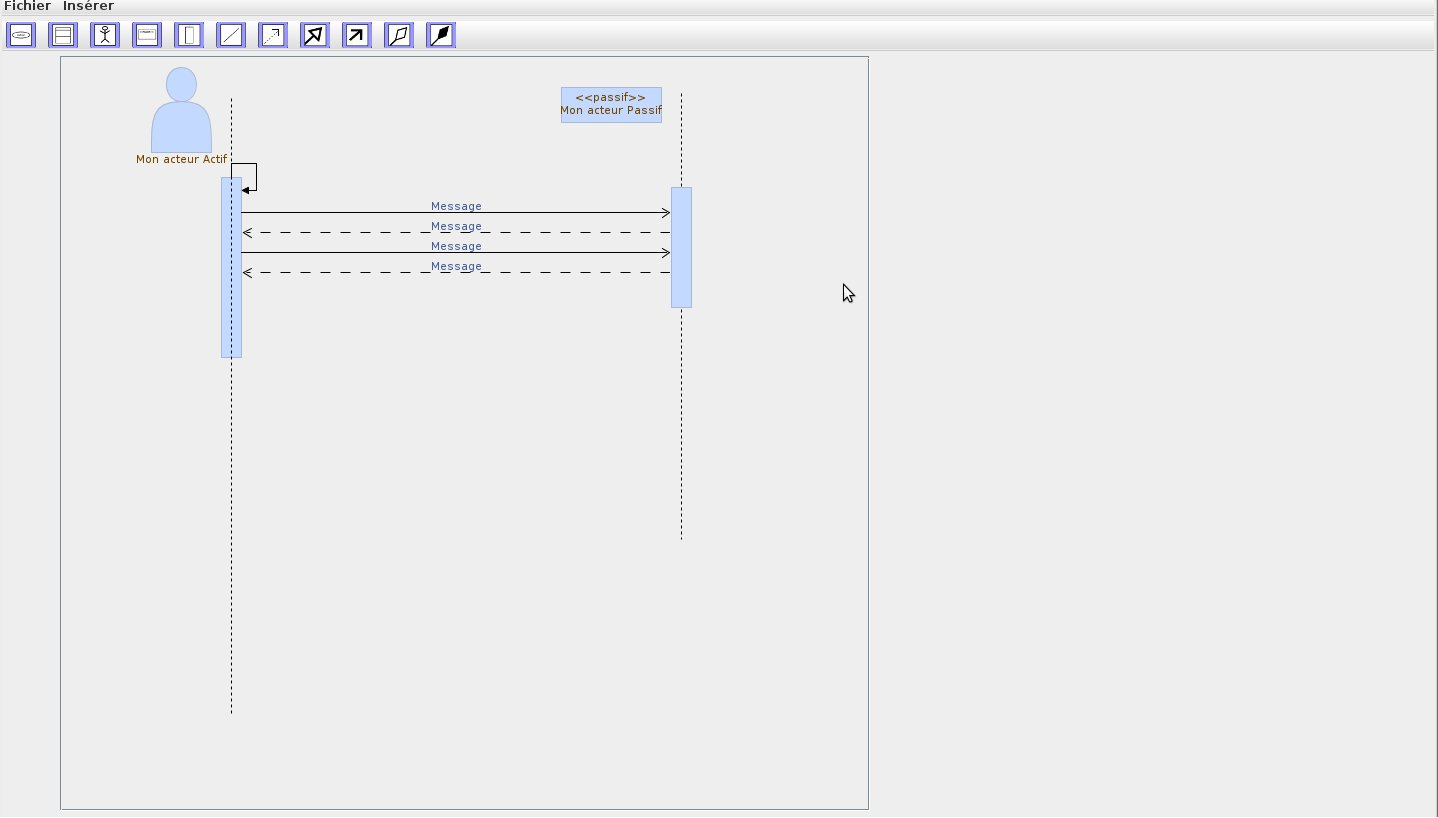
\includegraphics[width=18cm]{validation5.jpg}
			\caption{Création d'un diagramme de séquence simple}
			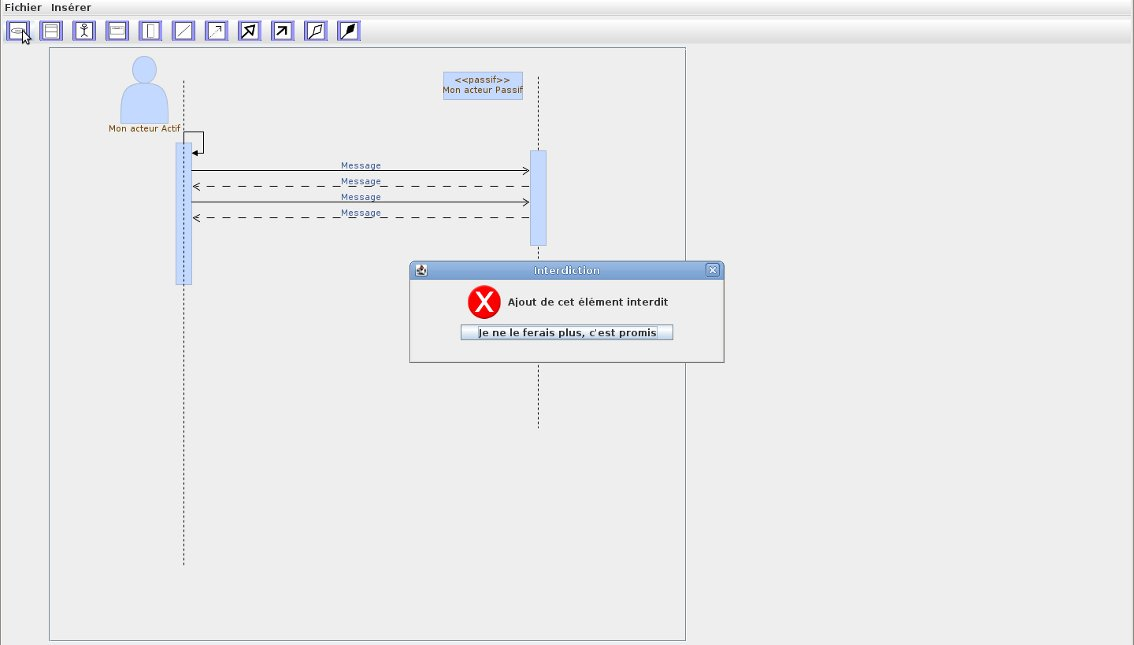
\includegraphics[width=18cm]{validation6.jpg}
			\caption{Validation de l'interdiction d'ajouter des éléments non autorisés}
		\end{figure}
		\newpage
			\begin{figure}[H]
				\section{Les tests d'intégration}
					\begin{flushleft} Nous avons créer un diagramme sans aucune contrainte, tous les éléments pouvant donc être reliés entre eux. \end{flushleft}
					\centering
					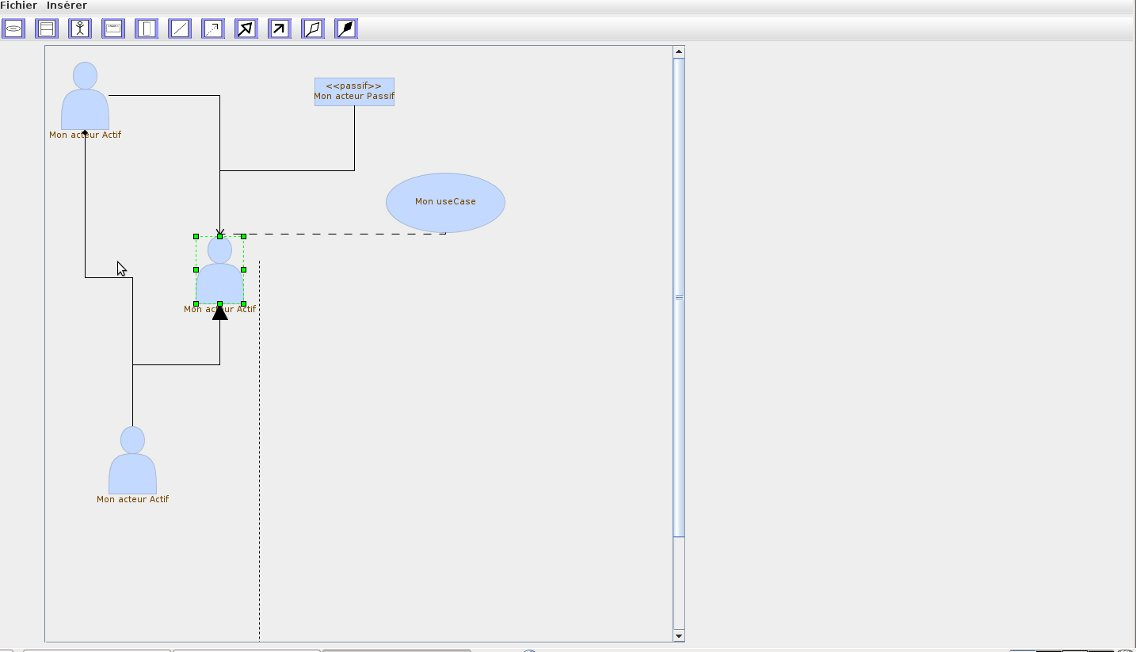
\includegraphics[width=18cm]{integration1.jpg}
					\caption{Diagramme sans aucune contrainte}
				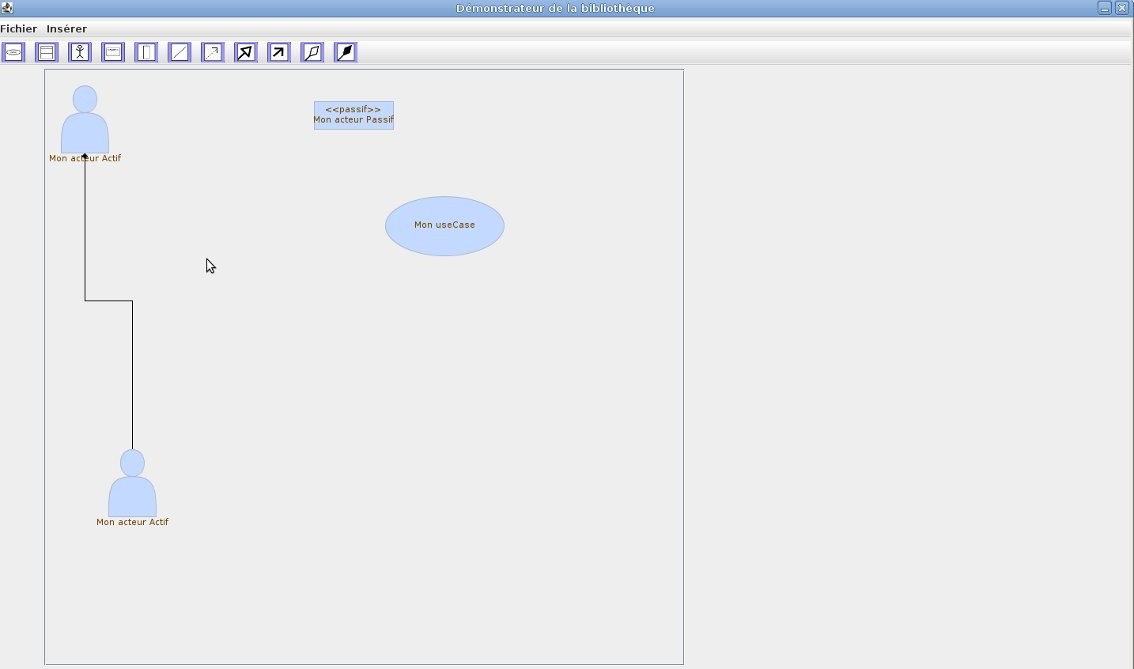
\includegraphics[width=18cm]{integration2.jpg}
				\caption{Le même diagramme après suppresion de l'acteur au centre}
			\end{figure}
			\begin{figure}[H]
				\section{Les tests unitaires}
				\subsection{Création des tests}
				\begin{flushleft}
					Nous avons donc créer des tests unitaires \texttt{JUnit}, une classe de test pour une classe à tester. Chaque méthodes doivent être testés, 
					avec un ou plusieurs tests.\\
					Vous pouvez avoir les détails des tests unitaires avec la documentation en Annexe \ref{junitdoc} page \pageref{junitdoc}.
				\subsection{Résultat des tests}
				Après lancement des tests unitaires, ils sont tous passéss. Nous pouvons donc en conclure que les différents modules de la bibliothèque UML fonctionnent. 
				\end{flushleft}
				\centering
				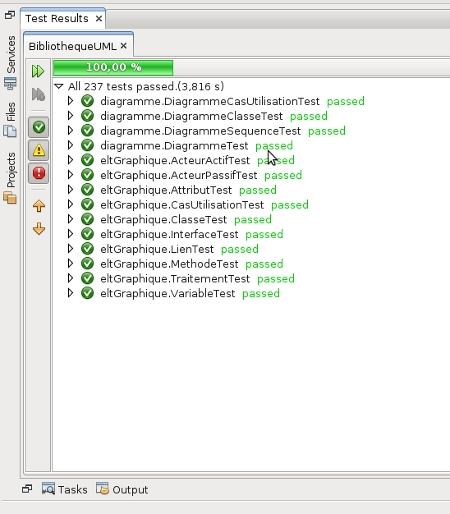
\includegraphics[width=9.75cm]{junitPassed.jpg} 
			\end{figure}
			\newpage
	\section{Le test de charge}
	\subsection{Création du test}
	Le test de charge à été effectuée en créant les éléments graphiques répértorié dans les plans de tests. Voici le code permettant d'effectuer ce tests:
	\lstinputlisting[language=Java, caption=Code du test de charge]{ChargeTest.java}
	\subsection{Résultat du test}
	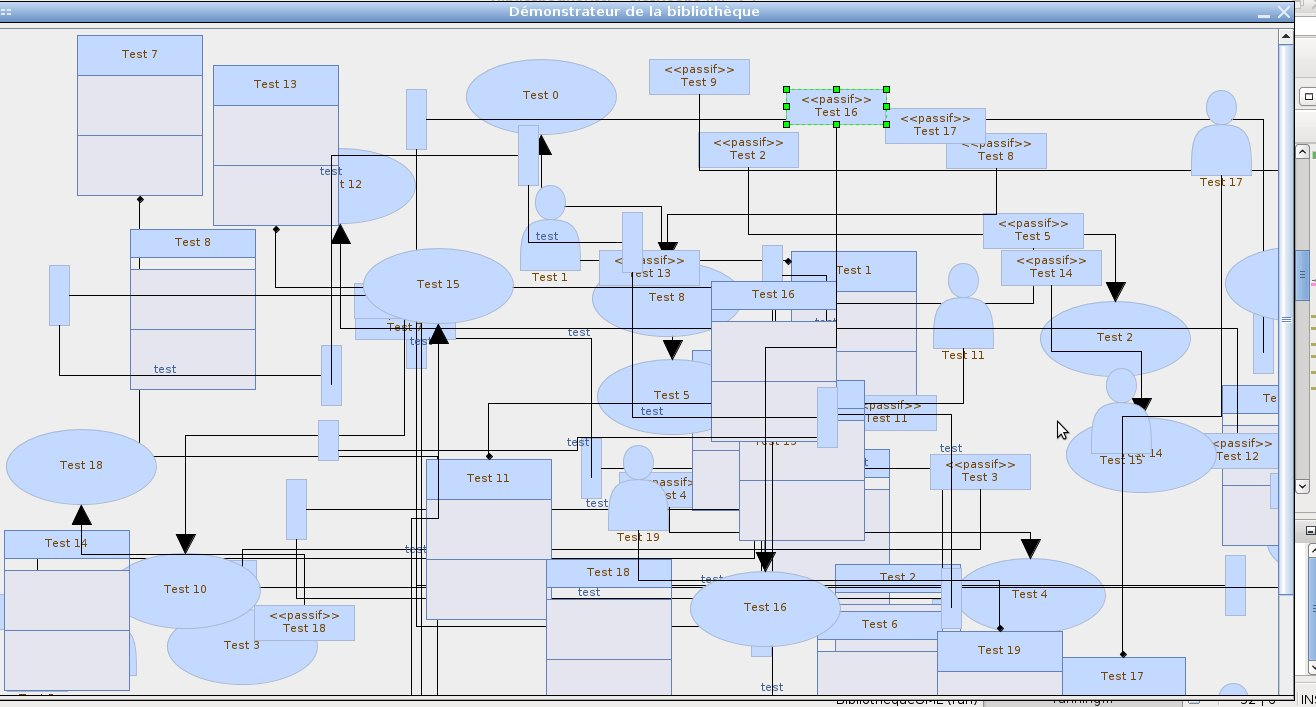
\includegraphics[width=25cm, angle=90]{testCharge.jpg}
	\closeout\glossaireVar
	\appendix	
	\chapter{Glossaire} \label{glossaire}
	\begin{sortedlist}
		\chapter {Glossaire}

	\end{sortedlist}

	\chapter{Documentation des tests unitaires}
	\label{junitdoc}
	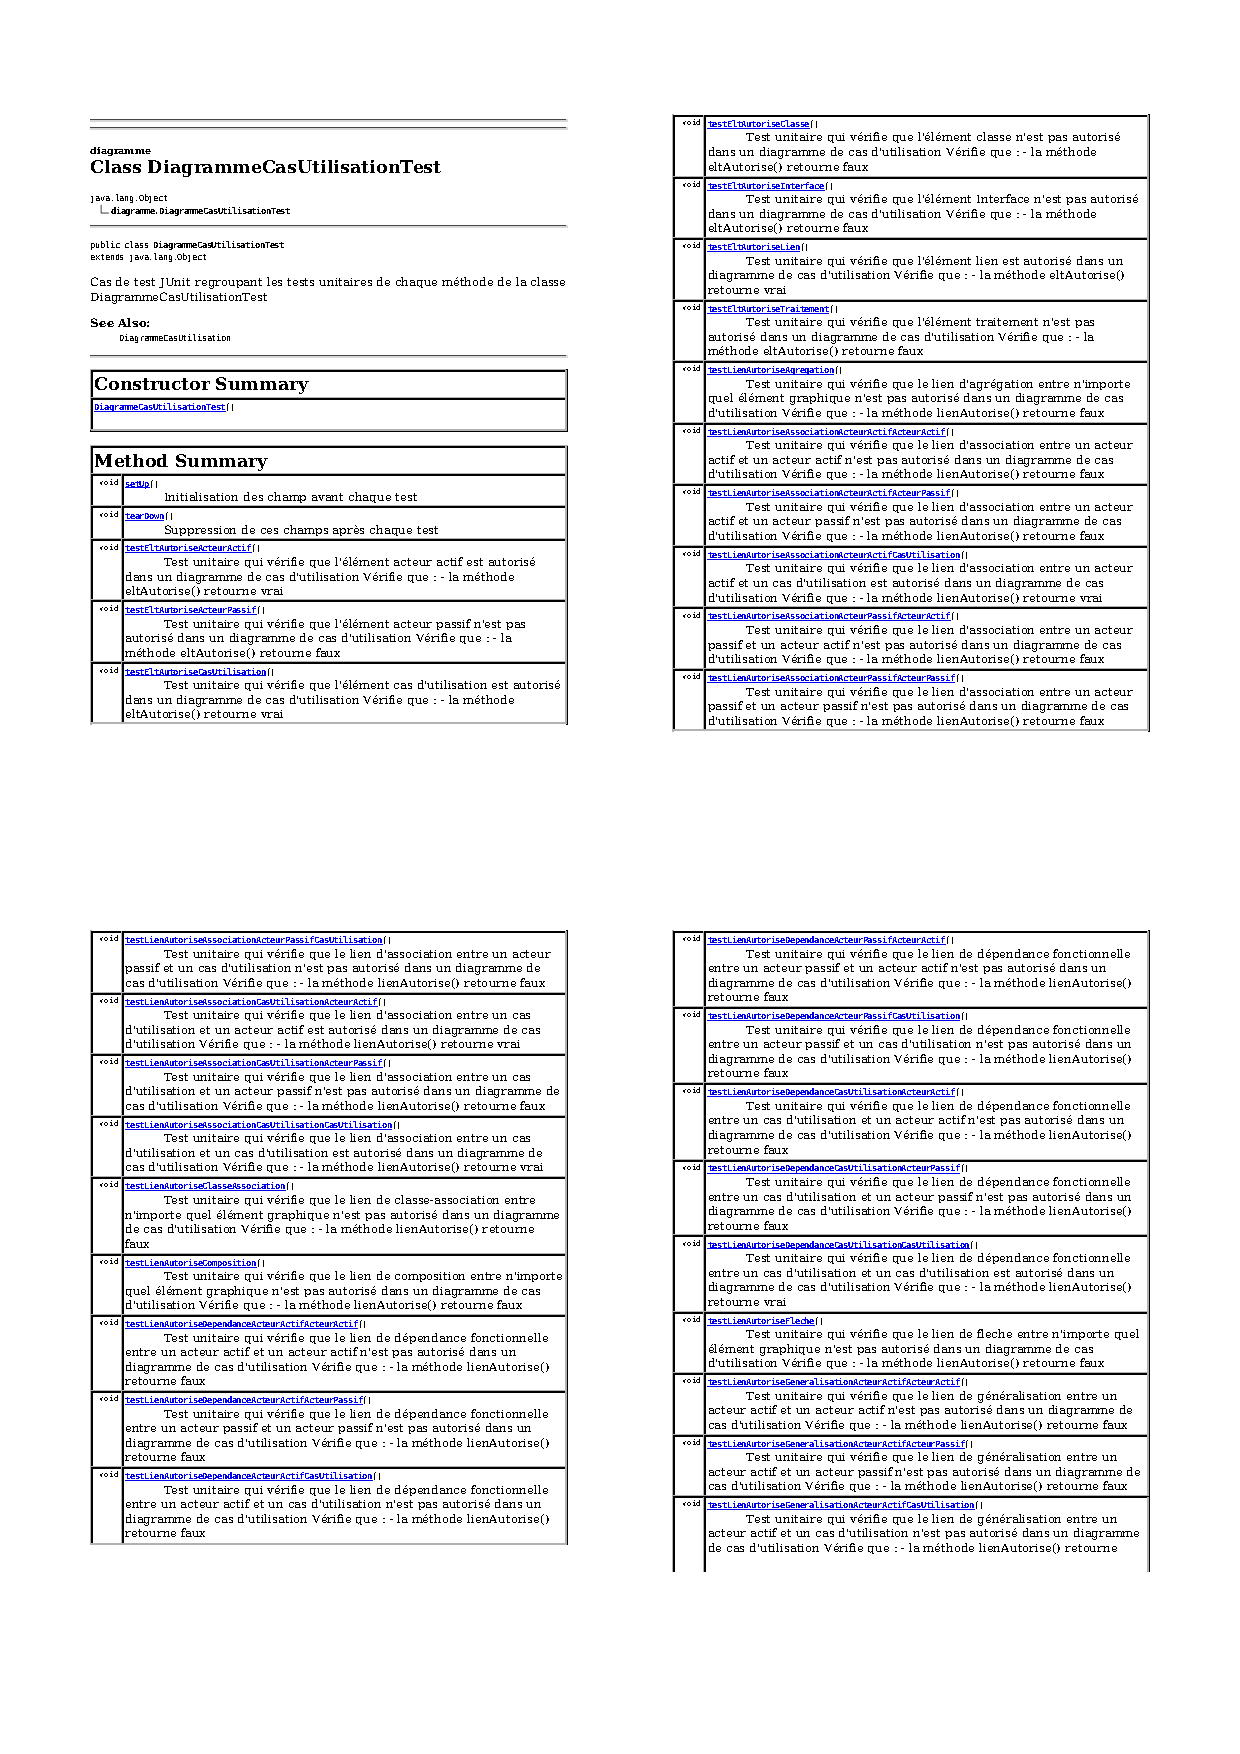
\includepdf[page=1-23]{docJUnit.pdf}
\end{document}
